% file:    Appendix-B-LQE.tex
% date:    July 27, 2005
% author:  Larry Eifler 
%    

% ==========Appendix B 

\addappendixline{EXAMPLES OF POSTSCRIPT CODING}
\thispagestyle{empty}

\null
\vspace{3.25in}
\begin{center}
  APPENDIX B \\
  EXAMPLES OF POSTSCRIPT CODING
\end{center}
\newpage

\thispagestyle{plain} 

\typeout{EXAMPLES OF POSTSCRIPT CODING}



The PostScript code for 
a modified y\={\i}ny\'{a}ng or  t\`{a}ij\'{\i}t\'{u} drawing 
is presented in  Figure \ref{YinYangCode}.  This code 
produced the drawing in Figure \ref{YinYangDrawing}.  

\begin{figure}[hbt]
\renewcommand{\arraystretch}{0.65}
\small
\begin{center}
\begin{tabular}{|l|}
\hline \\
\verb+  %!PS-Adobe-3.0 EPSF-3.0                           +\\ 
\verb+  %%BoundingBox: 149 249 471 571                    +\\ 
\verb+  %%Title:                                          +\\      
\verb+  %%Creator: Larry Eifler                           +\\ 
\verb+  %%CreationDate:(1/5/94)                           +\\ 
\verb+  %%EndComments                                     +\\     
\verb+                                                    +\\ 
\verb+  %   -- Procedures --                              +\\ 
\verb+  /Lines{                                           +\\ 
\verb+  40 20 120 { 20 moveto 0 120 rlineto } for         +\\ 
\verb+  30 20 130 { 20 exch moveto 120 0 rlineto } for    +\\ 
\verb+  }def                                              +\\ 
\verb+  %   -- Main Program --                            +\\ 
\verb+  150 250 translate      2 2 scale                  +\\ 
\verb+  1 setlinewidth  0.5 setgray                       +\\ 
\verb+  0 0 moveto                                        +\\ 
\verb+  160 0  lineto 160 160 lineto 0 160 lineto         +\\ 
\verb+  closepath fill                                    +\\  
\verb+  0 setgray  80 80 60 0 360 arc clip fill           +\\  
\verb+  1 setgray Lines stroke                            +\\ 
\verb+  80 50 10 0 360 arc fill                           +\\ 
\verb+  80 110  30  90 270 arc                            +\\ 
\verb+  80  50  30  90 270 arcn                           +\\ 
\verb+  80  80  60 270  90 arc clip fill                  +\\ 
\verb+  0 setgray Lines stroke                            +\\ 
\verb+  80 110 10 0 360 arc fill                          +\\  
\verb+  showpage                                          +\\ 
\verb+  %%EOF                                             +\\ 
  \\   \hline                      
\end{tabular}
\end{center}          
\caption{PostScript code for a yin/yang drawing }
\label{YinYangCode}
\end{figure}


\clearpage
  
%
\begin{figure}[htb] 
\begin{center}
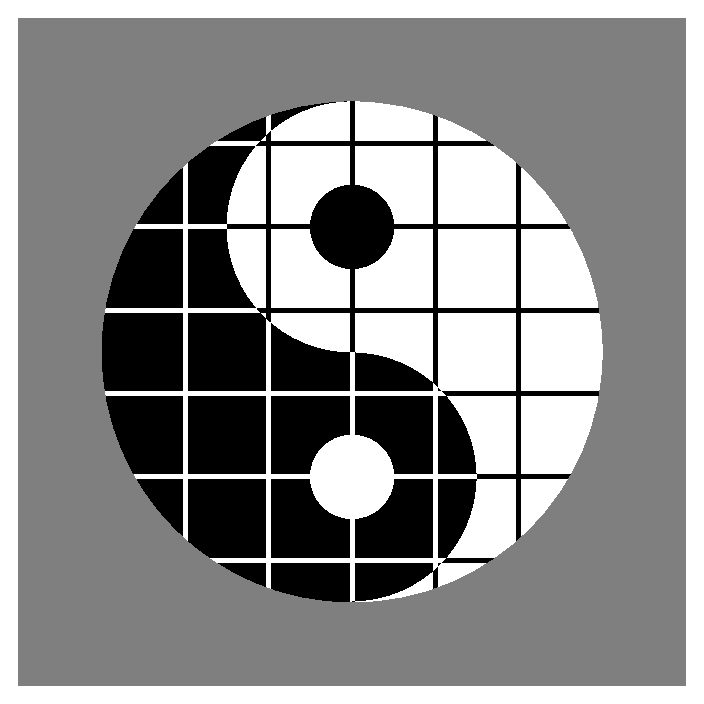
\includegraphics{YinYang.eps}
\end{center}
\caption{A whimsical yin/yang}
\label{YinYangDrawing}
\end{figure}
%


\clearpage
\endinput

